\section{ResNet18}
Jednym z największych problemów w uczeniu sieci konwolucyjnych
jest problem znikającego gradientu (ang. vanishing gradient). Polega
on na tym, że podczas uczenia sieci, propagowane gradienty stają się
coraz mniejsze, co prowadzi do tego, że w końcu stają się zbyt małe,
aby mogły skutecznie aktualizować wagi sieci. Problem ten zapobiega
budowaniu naprawdę głębokich sieci konwolucyjnych, które są
w stanie uczyć się złożonych reprezentacji danych.
\\

Rozwiązanie tego problemu zostało zaproponowane w pracy \cite{he2016deep}.
Autorzy zaproponowali architekturę sieci, w której podzielili sieć
na bloki, które mają połączenia rezydualne (wektor wejściowy jest dodawany
do wektora wyjściowego bloku). Połączenia te pozwalają na propagowanie
gradientów przez sieć, co zapobiega problemowi jego zanikania. Znane są różne
warianty tej architektury, które różnią się liczbą bloków oraz liczbą warstw (co można
zaobserwować na Rysunku \ref{fig:resnet_block}).
\begin{figure}[H]
  \centering
  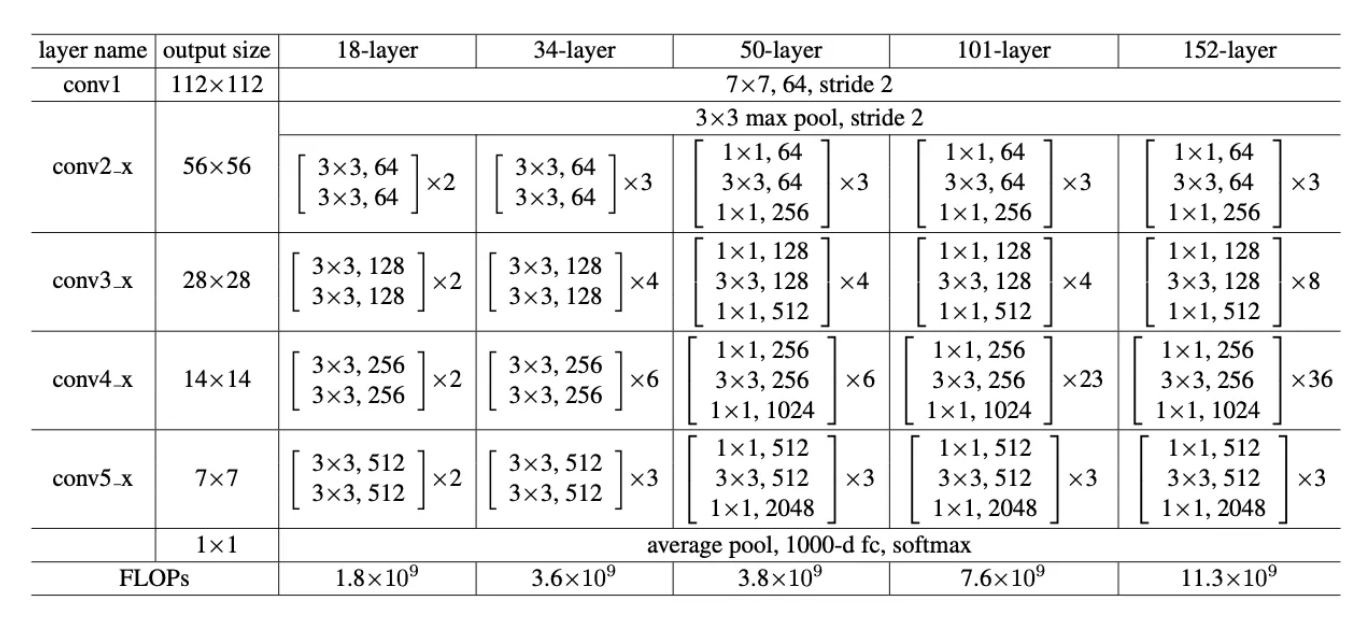
\includegraphics[width=0.8\textwidth]{ResNet/resnets.png}
  \caption{Różne warianty architektury ResNet. \cite{he2016deep}}
  \label{fig:resnet_block}
\end{figure}
W naszym projekcie wykorzystaliśmy wariant ResNet18, ponieważ jest on stosunkowo
mały, co pozwala na szybsze uczenie, a jednocześnie zapobiega przeczuczeniu modelu.
Przyjrzyjmy się bliżej tej architekturze. Na początku sieci znajduje się warstwa
konwolucyjna, która służy do wstępnego przetworzenia danych wejściowych. Następnie
znajduje się warstwa MaxPooling, która służy do zmniejszenia rozmiaru danych. Po niej znajdują
się 4 bloki, które składają się z dwóch warstw konwolucyjnych wraz z batch normalization oraz funkcją
aktywacji ReLU. W każdej z tych warstw znajduje się wspomniane wcześniej połączenie rezydualne.
Na samym końcu sieci znajduje się warstwa global average pooling, która służy do zamiany wektora z każdego kanału na
pojedynczą wartość, a następnie warstwa gęsta, która będzie służyła do klasyfikacji danych (w naszym przypadku
mamy tylko jedną klasę, bo jest to problem binarnej klasyfikacji).